\documentclass[12pt,a4paper]{book}
\newcommand\tab[1][1cm]{\hspace*{#1}}
\usepackage{amsmath,amsthm,amssymb,graphicx,hyperref}
\usepackage[left=1.2in,right=1.2in,top=1in,bottom=1in]{geometry}
\usepackage[romanian, english]{babel}
\usepackage[english]{babel}
\usepackage{xcolor}
\usepackage{paralist}
\usepackage{lipsum} 
\RequirePackage{hyphenat}
\usepackage{algorithmic, algorithm}
\usepackage[inline]{enumitem}
\usepackage[acronym]{glossaries}
\usepackage{hyperref}
%\usepackage{...insert other packages here...}
\newtheorem{thm}{Theorem}[section]
\newtheorem{lem}[thm]{Lemma}
\theoremstyle{definition}
\newtheorem{defn}{Definition}[section]
\theoremstyle{remark}
\newtheorem{rem}{Remark}[section]
\newtheorem{exmp}{Example}[section]


\makeglossaries

\newacronym{gcd}{GCD}{Greatest Common Divisor}

\newacronym{lcm}{LCM}{Least Common Multiple}

\begin{document}
\sloppy

\thispagestyle{empty}

\begin{center}
    \begin{figure}[h!]
        \vspace{-20pt}
        \begin{center}
            
\includegraphics[width=100pt]{img/FMI-03.png}
        \end{center}
    \end{figure}


    {\large{\bf WEST UNIVERSITY OF TIMI\c SOARA

        FACULTY OF MATHEMATICS AND COMPUTER SCIENCE

        BACHELOR:  Computer Science in romanian}}

    \vspace{120pt}
    {\huge {\bf BACHELOR THESIS}}

    \vspace{160pt}
\end{center}

{\large\noindent{\bf SUPERVISOR:
    \hspace{172pt} GRADUATE: }

\noindent Lect. Dr. Liviu Mafteiu-Scai\hfill
\noindent Sorin-Ionu\c t Rosalim
}

\vfill
\begin{center}
    {\bf TIMI\c SOARA

        2023}
\end{center}
\newpage
\thispagestyle{empty}
\begin{center}
    {\large{\bf WEST UNIVERSITY OF TIMI\c SOARA

            FACULTY OF MATHEMATICS AND COMPUTER SCIENCE

            BACHELOR:  Computer Science in English}}

    \vspace{200pt}
    {\huge {\bf Development of an augmented reality app as an interactive tool}}

    \vspace{153pt}
\end{center}

{\large\noindent{\bf SUPERVISOR:\hfill GRADUATE:}

\noindent Lect. Dr. Liviu Mafteiu-Scai\hfill
\noindent Sorin-Ionu\c t Rosalim}


\vfill
\begin{center}
    {\bf TIMI\c SOARA

        2023}
\end{center}

\newpage
\normalsize{}

\section*{Abstract}
In this paper, we present a novel approach to the problem of augmenting the real world with digital content. We propose a new method for augmenting the real world with digital content using QR codes. We present a proof of concept of our approach, and we discuss the potential of our approach in the context of education. The augmentate reality is a tool for improving the learning process. We also discuss the potential of our approach in the context of augmented reality. We conclude by discussing the future work that we plan to do in this area.
\newline
\newline
În această lucrare, prezentăm o abordare nouă a problemei dezvoltarii lumii reale cu conținut digital. Vă propunem o nouă metodă de dezvoltarii a lumii reale cu conținut digital folosind coduri QR. Prezentăm o dovadă de concept a abordării noastre și discutăm potențialul abordării noastre în contextul educației. De asemenea, discutăm potențialul abordării noastre în contextul realității augmentate. Încheiem prin a discuta despre dezvoltarea viitoare pe care intenționăm să o facem în acest domeniu.

\section*{Meeting Schedule}
The Meeting Schedule with my Coordinator is not fixed because also I am working besides university. We are keeping in touch using emails. We look forward to meet at least once a week.
\tableofcontents
\listoffigures

\chapter{Introduction}\label{cap:introduction}

\section{Project Theme}
Augmented Reality is a technology combining the virtual and physical worlds, allowing digital content to be added on top of the physical world.
\ac{AR} relies on device sensors to detect the users' surroundings, position and orientation. \ac{QR} codes are a type of barcode; they are predominantly used to store information such as text, links, and images and are easy to share.

By combining these two technologies, we can create a new way of accessing digital content and interact with newly accessed information in the real world. This technology gives users the power of enhanced perception while accessing digital content that can be used for entertainment or didactic purposes.


\section{Theme Relevance}
The topic of \ac{AR} is relevant because it can be implemented and used in a multitude of domains. This technology is already used in the following domains:
\begin{itemize}
    \item \ac{3D} printing - \ac{AR} is used to visualise the \ac{3D} model of the object that will be printed.
    \item Architecture - \ac{AR}is used to visualise the \ac{3D} model of a building or a house.
    \item Automotive - \ac{AR} is used for navigation and to display map information.
    \item Publicity - \ac{AR} is used to lunch novel marketing campaigns and interact with digital content.
\end{itemize}


Augmented reality is an interactive experience that recently became more accessible to the world with the help of the smartphone. Most smartphones have the necessary hardware to run \ac{AR} applications. This \ac{AR} applications give their users a new perspective on the digital content that they are accessing.
\pagebreak

\ac{QR} codes are two-dimensional matrix barcodes that are easily scanned by a smartphone camera. They were first used for tracking parts in vehicle manufacturing. Nowadays, they are used in a wide variety of domains, such as:
\begin{itemize}
    \item Virtual stores - \ac{QR} codes are used to display information about the products.
    \item Online payments - \ac{QR} codes are used to store payment information.
    \item WI-FI access - \ac{QR} codes are used to store WI-FI access information.
    \item Augmented reality - \ac{QR} codes are used in some \ac{AR} applications to determine the positions of objects in \ac{3D} space.
\end{itemize}


\section{Project Aim}
The AR topic was chosen because this technology has many applications in different fields. The immersive experiences of \ac{AR} allow people to do interactive activities.

The primary objective is to develop a highly functional mobile application that utilises \ac{AR} and allows users to scan \ac{QR} codes. Then using the available models in the \acf{AR} mode to move, resize, rotate and interact with them.

The application is developed for the Android platform. To accomplish this, Android Studio \ac{IDE} was utilized alongside Google's ARCore \ac{SDK}, which provides powerful augmented reality capabilities. In order to store the \ac{3D} models, we make use of the Google Buckets service, which offer reliable and easy-to-use storage solution. This application will have a user-friendly interface that is both simple and intuitive, ensuring that users can easily navigate and interact with all the features.

One of the key highlights of this application is its interactive functionality for some \ac{3D} models. Users can trigger engaging animations or explore different states of the model by simply touching a button. This innovative approach offers users a fresh way to access digital content and actively participate in the learning and discovery process. It opens up exciting new possibilities for users to create, learn and explore.

To ensure a seamless experience for all users, the application will undergo rigorous testing on multiple Android devices. This will help identify and address any compatibility issues that may arise. Once the application has been thoroughly tested, it will be published on the Google Play Store, making it available to a wide audience.

\newpage
\section{Author's contribution}
I have utilized my knowledge and expertise to develop a mobile application that incorporates the Google ARCore \ac{SDK}, a \ac{QR} code scanner and the Google Buckets service. Through the integration of these technologies, I have created a novel approach to accessing and interacting with digital content. This application empowers users with an augmented perception of their surroundings, enabling them to engage with digital content using their smartphones.


The application is able to load the interaction module specific for each \ac{3D} model. The interaction module will be a simple animation or a different state of the \ac{3D} model. For example, if the \ac{3D} model is a LEGO car, the interaction module will be a simple guide for assembling the LEGO car. If the model is related to a geometrical shape, related to the school geometry curriculum, the interaction module will display a different perspective of the \ac{3D} model, for example, if the \ac{3D} model is a cube, the interaction module will display only the cube's edges.





\chapter{Application description}\label{chapter:appdescription}


\section{Requirements}
The application can be used in different area of application. The main requirement is to have a smartphone with a camera and a QR code reader. The application is available for Android and iOS. The application is available for free on the Google Play Store and the Apple App Store. The application is available in English and Romnian. The users will be able to import any model in the application using the QR code.

\section{Description}
\pagebreak
\section{Diagrams}
\subsection{Use cases}
Each user that has a smartphone capable to run the AR moduls should be able to use the app. If the user has models already imported he/she can use the app without any connection to the internet. If the user wants to import a new model he/she will need to have an internet connection. The user will be able to import a model using the QR code. The user will be able to see the model in AR mode. The user will be able to see the guide of the model. The user will be able to see the list of all the models that he/she has imported. The user will be able to delete a model from the list of models. The user will be able to see the list of all the models that he/she has imported. The user will be able to delete a model from the list of models.
\begin{figure}[h!]
    \begin{center}
        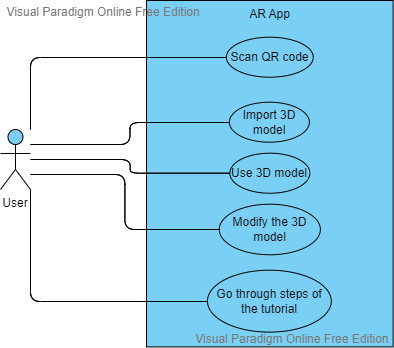
\includegraphics{img/InitialUseCase.png}
        \caption{Initial use case}
        \label{fig:InitialUseCase}
    \end{center}
\end{figure}
\pagebreak

\subsection{Sequence diagram}
TEXT TO BE ADDED
\begin{figure}[h!]
    \begin{center}
        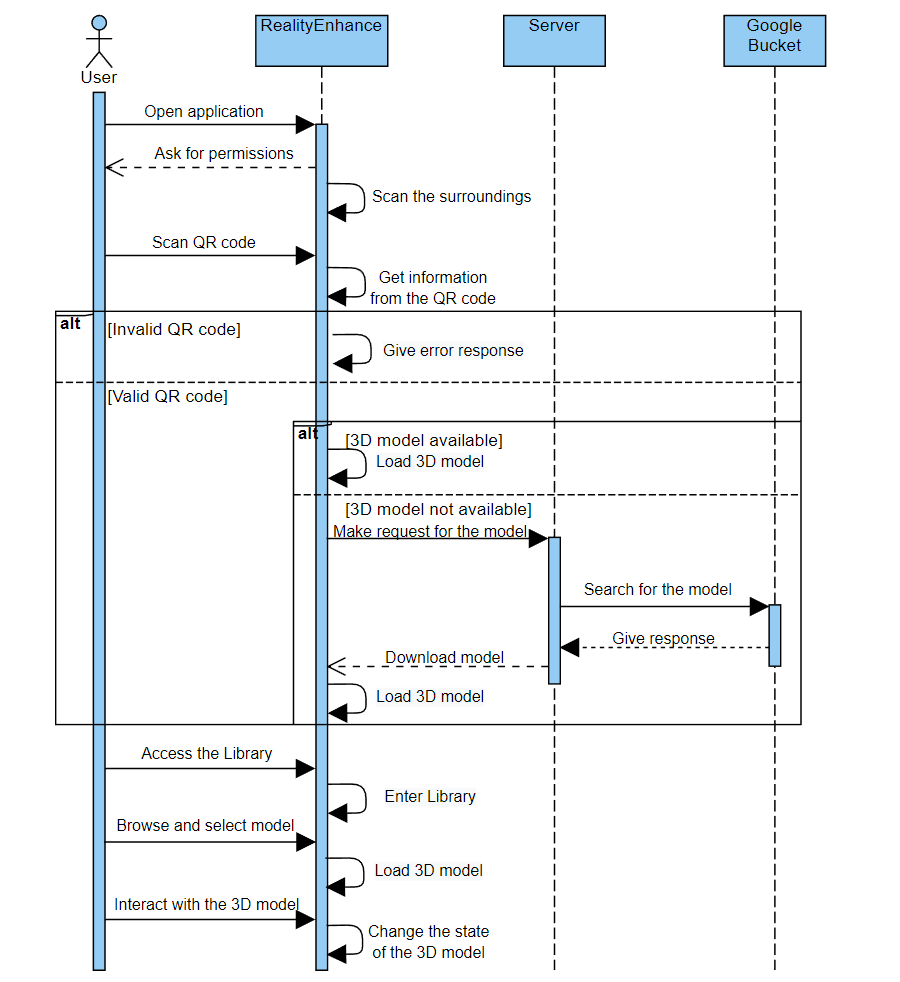
\includegraphics{img/SequenceDiagram.png}
        \caption{Sequence diagram}
        \label{fig:SequenceDiagram}
    \end{center}
\end{figure}

\section{Features}
\subsection{Import model}
\subsection{See model in AR}
\subsection{See guide}
\subsection{See list of models}
\subsection{Delete model}
\subsection{Load model from library}
\subsection{Create a scene}


\section{Architecture}
The application will be developed using the Android Studio IDE. The application will be developed using the Java programming language. The application will use the Google ARCore framework. The application will use the Firebase cloud database to store the models. The application will use the QR code reader to import the models. The application will use the Google Vision API to recognize the QR code.
\begin{figure}
    \begin{center}
        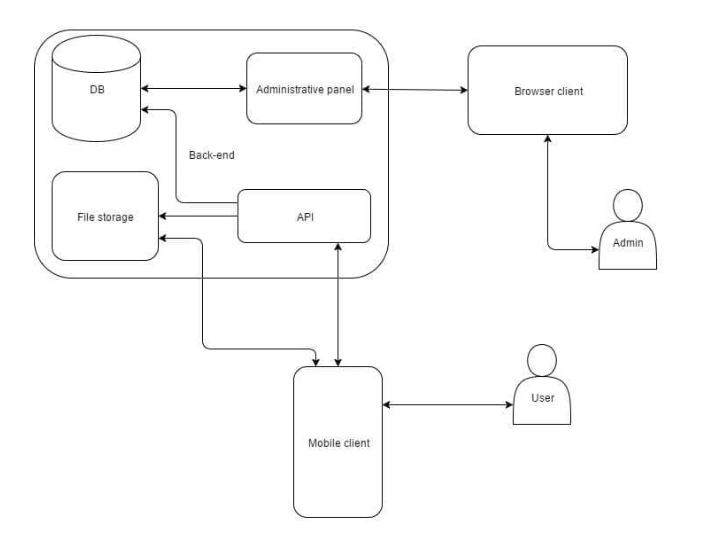
\includegraphics{img/architecture.png}
        \caption{Architecture}
        \label{fig:architecture}
    \end{center}
\end{figure}

\begin{itemize}
    \item \textbf{Android Version 7.0+} - to use the application on the phone
    \item \textbf{Android Studio} - IDE for Android development
    \item \textbf{Firebase} - Cloud DataBase for where the models will be retrieved
    \item \textbf{Java} - Programming language
    \item \textbf{Google ARCore} - AR framework
\end{itemize}

\section{Implementation}

\section{Testing}

\section{Deployment}

\section{Maintenance}



\chapter{User Manual}\label{cap:evaluation}
\section{Graphical overview of RealityEnhance}
We will now go through some of the application's graphical user interfaces. This should give a summary of the fundamental flows present in the program and accommodate the user with regard to the interface.
\pagebreak

\subsection{App start page}
The fisrt thing any user will see when they lounch the app on their phone is the loading page. This page is a simple loading screen that will be displayed while the app is loading. In the loading phase the app will check if the user is able to run the app on their phone and if the phone has the necessary sensors to run the app. If the user is able to run the app, the app will load the main page. If the user is not able to run the app, the app will display a message that the user is not able to run the app on their phone.
\begin{figure}[h!]
    \begin{center}
        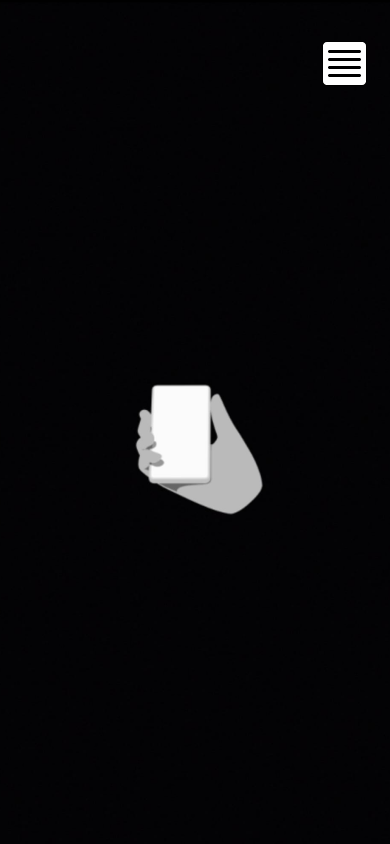
\includegraphics[scale=0.5]{img/App_mock/iPhone 14 - 1.png}
        \caption{Loading page}
        \label{fig:loading-page}
    \end{center}
\end{figure}
\pagebreak


\subsection{App burger button}
The burger button is a button that is present on every page of the app. It is used to open the side menu. The side menu is used to navigate through the app. In the burger button we have access to the following options: QR scanner, Library, and EXIT.
The QR scanner is used to scan a QR code and load a 3D model and a guide into the user's smartphone. The Library is used to display all the 3D models that the user has scanned. The EXIT button is used to exit the app.
\begin{figure}[h!]
    \begin{center}
        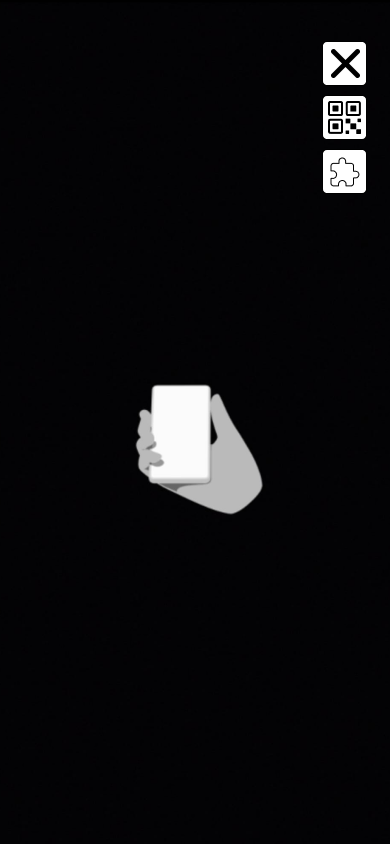
\includegraphics[scale=0.5]{img/App_mock/iPhone 14 - 2.png}
        \caption{Burger button menu}
        \label{fig:burger-button}
    \end{center}
\end{figure}
\pagebreak

\subsection{QR scanner}
In this mode, on the user's screen will be displayed a camera view. The user will have to scan a QR code. The QR code will contain a link to a 3D model and a guide. The app will download the 3D model and the guide and will display them on the user's screen. The model loaded from the QR code will be ready to use without the need to enter the Library menu. The guide will be displayed on the user's screen and the user will have to follow the guide to assemble the 3D model.

\begin{figure}[h!]
    \begin{center}
        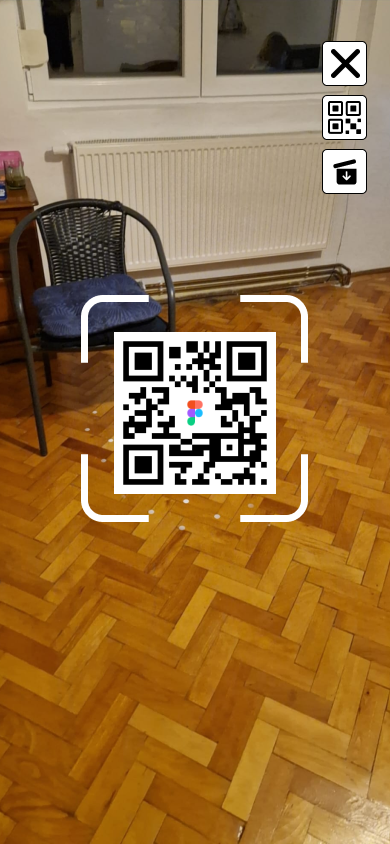
\includegraphics[scale=0.5]{img/App_mock/iPhone 14 - 3.png}
        \caption{QR scanner interface}
        \label{fig:qr-scanner}
    \end{center}
\end{figure}
\pagebreak

\subsection{QR valdiation}
If the QR code is valid, the app will display a message that the QR code is valid and will load the 3D model and the guide. If the QR code is not valid, the app will display a message that the QR code is not valid.

\begin{figure}[h!]
    \begin{center}
        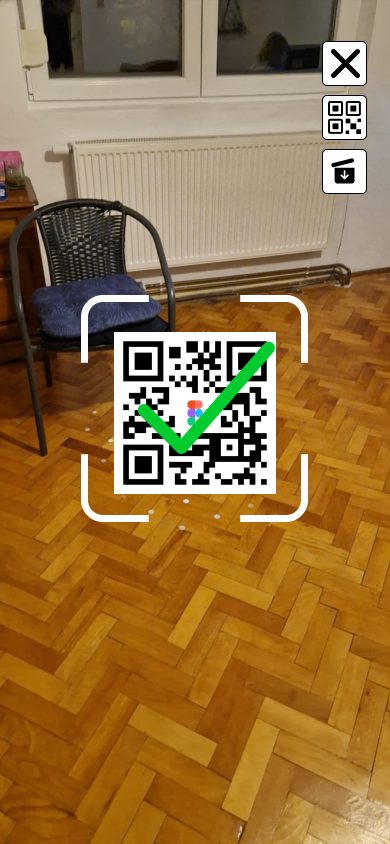
\includegraphics[scale=0.5]{img/App_mock/iPhone 14 - 4.png}
        \caption{QR code is valid}
        \label{fig:qr-valdiation}
    \end{center}
\end{figure}
\pagebreak

\subsection{AR vision}
After a model is loaded, the AR moduls will use the phone's camera to find out what is around the user. It will make a 3D model of the environment and will place the 3D model on top of the environment. The user will have a guide of the app is understanding the surroundings (a mesh of the planes will be displayed on the screen).
\begin{figure}[h!]
    \begin{center}
        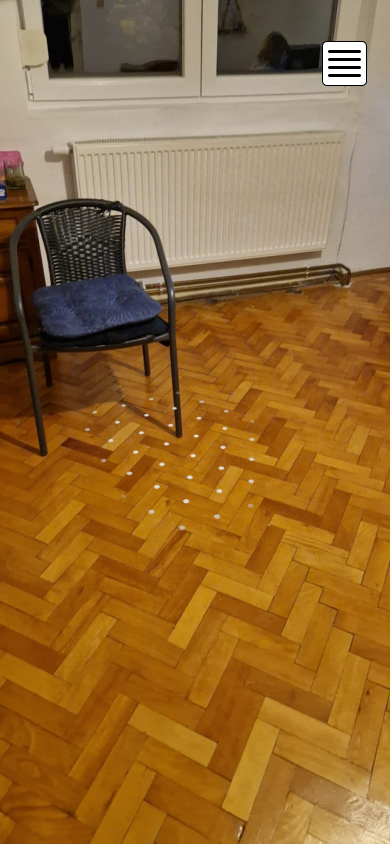
\includegraphics[scale=0.5]{img/App_mock/iPhone 14 - 5.png}
        \caption{AR vision interface}
        \label{fig:ar-vision}
    \end{center}
\end{figure}

\pagebreak

\subsection{Adding a model}
After the app has a basic understanding of the surroundings and a model loaded, the user can click on the screen to add an object to the scene. This object will be placed on the screen and the user will be able to move it around the screen. The user will be able to move the object around the screen by press-and-hold the object and moving phone around or draging the object with his/her finger across the screen. The user will be able to rotate the object by rotating the model using two fingers (like opening a bottlle cap(rotating clock-wised) or closing a bottlle cap(rotating counter-clock-wised)). The user will be able to scale the object by pinching the screen. The user is not bound to use just a single object. The user can add multiple objects to the scene and move them around the screen. The user will be able to add another object by clicking on the screen in a place where an object is not present.
\begin{figure}[!h]
    \begin{center}
        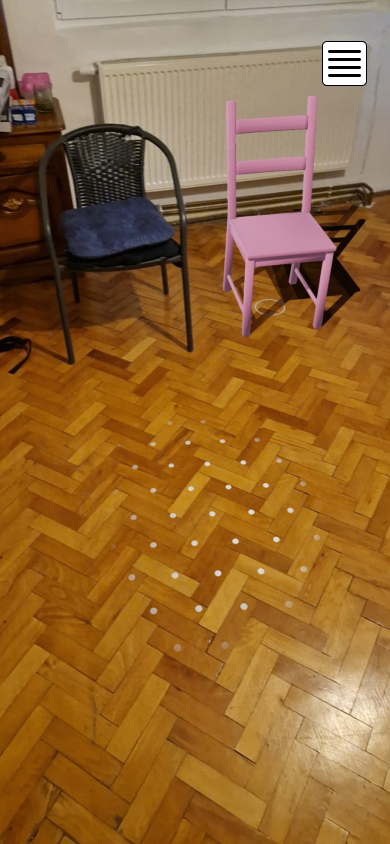
\includegraphics[scale=0.5]{img/App_mock/iPhone 14 - 6.png}
        \caption{Adding a model}
        \label{fig:add-a-model}
    \end{center}
\end{figure}
\pagebreak

\subsection{Removing a model}
The user will be able to remove the object by clicking and holding on the object and then clicking on the remove button. The user will be able to remove multiple objects at the same time by clicking on the reset all button.
\begin{figure}[h!]
    \begin{center}
        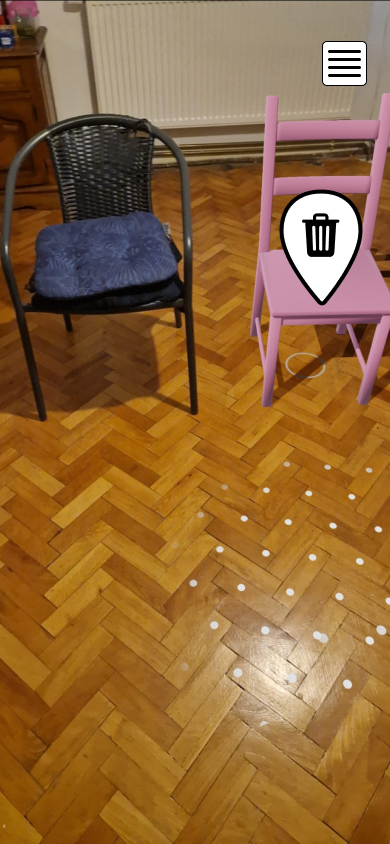
\includegraphics[scale=0.5]{img/App_mock/iPhone 14 - 7.png}
        \caption{Removing a model}
        \label{fig:remove-a-model}
    \end{center}
\end{figure}
\pagebreak


\begin{center}
    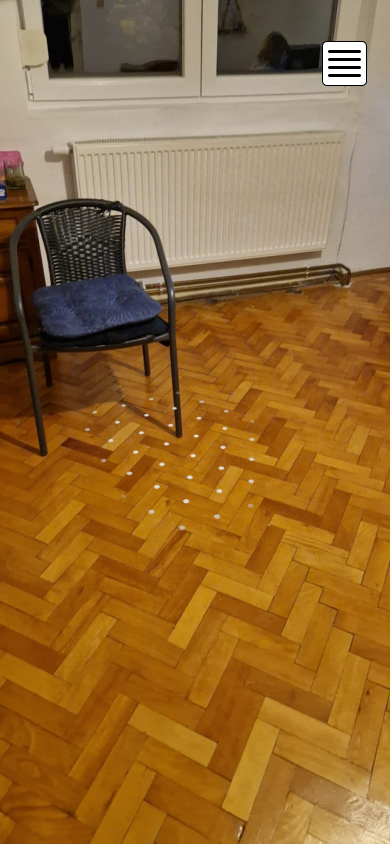
\includegraphics[scale=0.5]{img/App_mock/iPhone 14 - 8.png}
\end{center}
\pagebreak

\begin{center}
    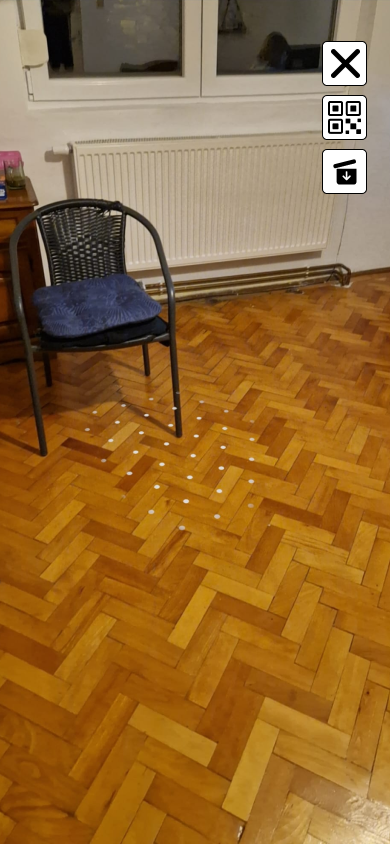
\includegraphics[scale=0.5]{img/App_mock/iPhone 14 - 9.png}
\end{center}
\pagebreak

\subsection{Library}
When the user clicks on the Library button in the burger menu, the app will display the Library interface. The Library interface will display all the 3D models that the user has scanned. The user will be able to select a model and load it into the AR vision mode. In the Library interface, the user can search for a model and add a model to the Library. The user can also delete a model from the Library.
\begin{figure}[h!]
    \begin{center}
        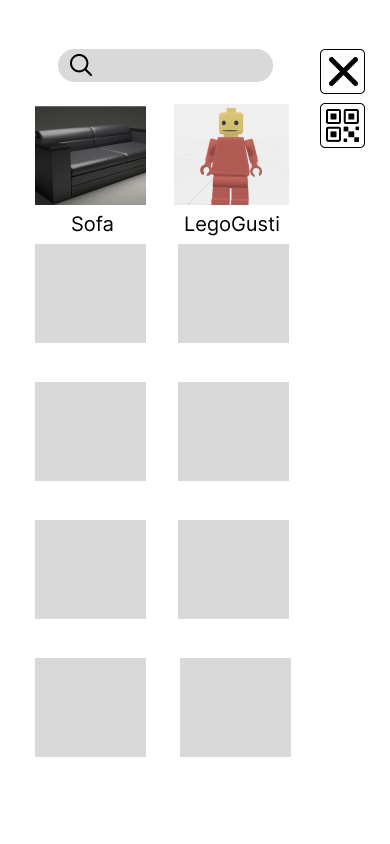
\includegraphics[scale=0.5]{img/App_mock/iPhone 14 - 10.png}
        \caption{Library interface}
        \label{fig:library}
    \end{center}
\end{figure}
\pagebreak

\subsection{Using multiple models at the same time}
The user will be able to use multiple models at the same time. The user will be able to add multiple models to the scene and move them around the screen. The user will be able to add another model by clicking on the screen in a place where an object is not present. The guide for assembling or building a model will be displayed on the screen when in the scene is present just one object.
\begin{figure}[h!]
    \begin{center}
        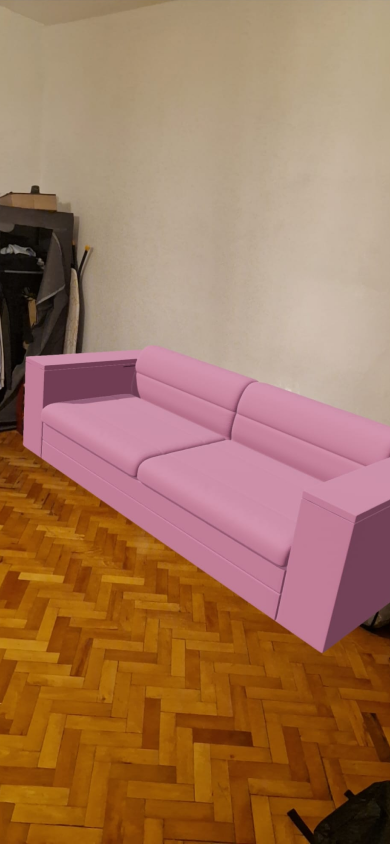
\includegraphics[scale=0.5]{img/App_mock/iPhone 14 - 11.png}
        \caption{Using multiple models}
        \label{fig:using-multiple-models}
    \end{center}
\end{figure}
\pagebreak

\section{Proof of concept}

\section{Domains of application}
\subsection{Interior designing}
\subsection{Outdoor designing}
\subsection{3D printing}
\subsection{Architecture}
\subsection{Pedagogical instrument}


\chapter{Implementation of the application features}\label{cap:aplicationfeatures}

\section{QR code-scanner}
The only way to import a new model is by scanning a QR code. The QR code contains the ID of the model. The application will check if the model is already in the local models' directory. If it is, it will load it from there, as shown in Figure \ref{fig:loadModelQR}. If it is not, it will proceed to download it from Google Bucket Storage.

\begin{wrapfigure}{r}{.5\textwidth}
    \centering
    \subfigure[loadModelQR]{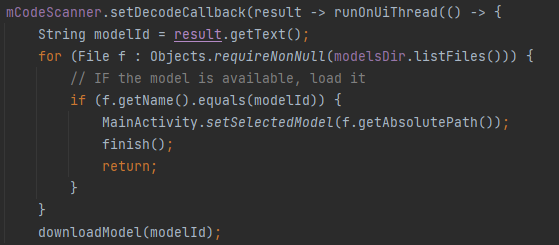
\includegraphics[width=0.5\textwidth]{img/code/loadModelQR.png}}
    \vspace{0.3cm}
    \subfigure[downloadModel] {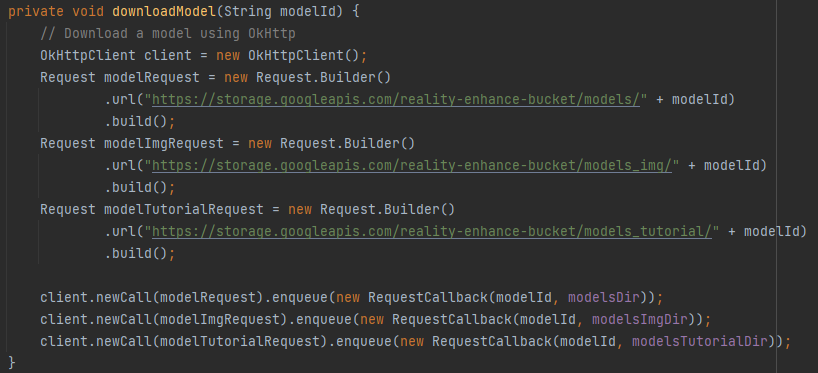
\includegraphics[width=0.5\textwidth]{img/code/downloadModel.png}}
    \caption{QR code-scanner methods}
    \label{fig:loadModelQR}
\end{wrapfigure}



Then the application will handle the response from Google Bucket Storage. If the response is successful, the model will be saved in the local models' directory and loaded in the \ac{AR} scene. If the response is not successful, the application will display an error message, as seen in Figure \ref{fig:onResponse}.


\begin{wrapfigure}{l}{.45\textwidth}
    \centering
    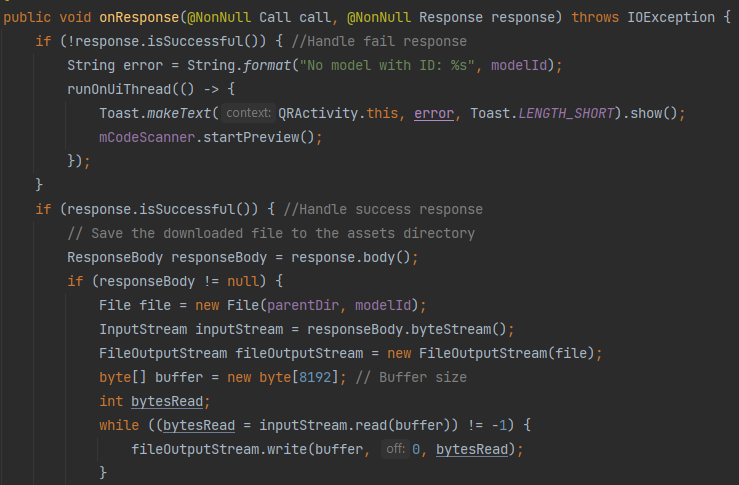
\includegraphics[width=0.45\textwidth]{img/code/onResponse.png}
    \caption{onResponse method}
    \label{fig:onResponse}
\end{wrapfigure}

\clearpage

\section{Load the starting models}
When the user starts the application, the method from Figure \ref{fig:tryMoveAssets} will be called.
\begin{figure}[H]
    \centering
    \subfigure{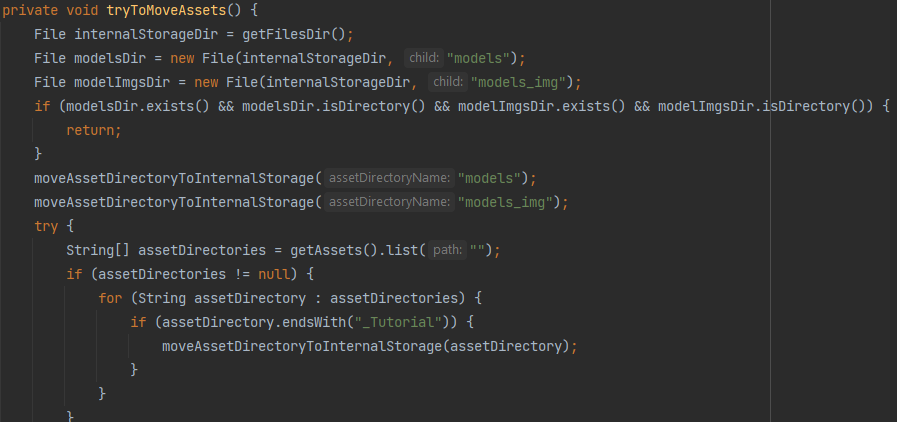
\includegraphics[width=0.8\textwidth]{img/code/tryMoveAssets.png}}
    \subfigure{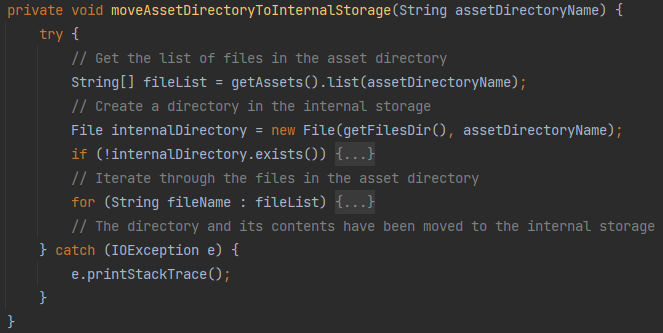
\includegraphics[width=0.6\textwidth]{img/code/moveAssets.png}}
    \caption{Move files from assets to local storage}
    \label{fig:tryMoveAssets}
\end{figure}


It will load the models from the assets directory to the local smartphone storage because the assets directory is read-only at runtime, and the application must store all the newly imported models at the same location. The method will check if the models are already in the local storage. If they are, it will load them from there. If they are not, it will copy them from the assets directory to the local storage.

\newpage
\section{Models' library}
In the Library Activity, the models will be displayed in two columns. This is done at the start of the activity, in the method from Figure \ref{fig:loadModels}. It will go through all the files from the local models' directory and it will create a new button for each file.

The buttons will have as background the image of the model. If the model does not have a background image, the button will have as background the name of the model. When the user clicks on a button, the model will be loaded in the \ac{AR} scene.

\begin{figure}[H]
    \centering
    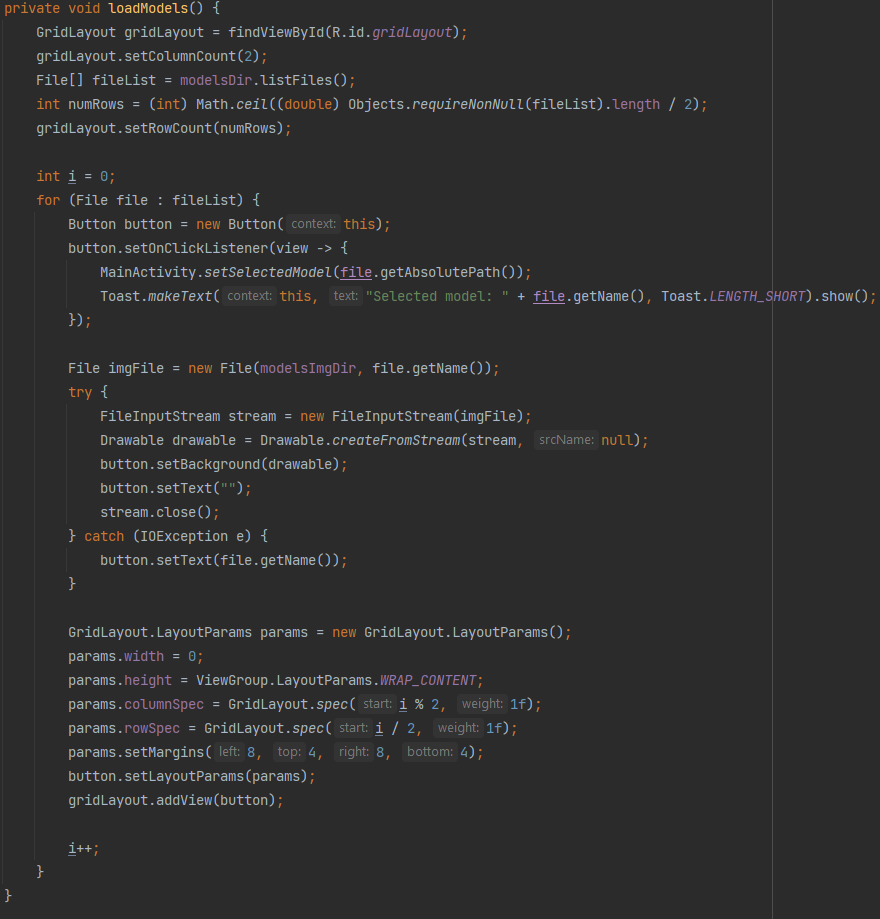
\includegraphics[width=0.8\textwidth]{img/code/loadModels.png}
    \caption{Load models in the library}
    \label{fig:loadModels}
\end{figure}

\newpage
\section{Interaction with  the models}
The user can interact with the models in the \ac{AR} scene by using the buttons on the screen and using smart gestures on the model. As seen in Figure \ref{fig:addModeltoScene}, when the user taps on the screen, the addModelToScene method will be called. It will check if the model has an interactive mode; if it does, it will activate the button responsible for the interaction with the model. If the model does not have an interactive mode, it will display a message to the user. Each time the user presses the interaction button, the model will change its state.

\begin{figure}[H]
    \centering
    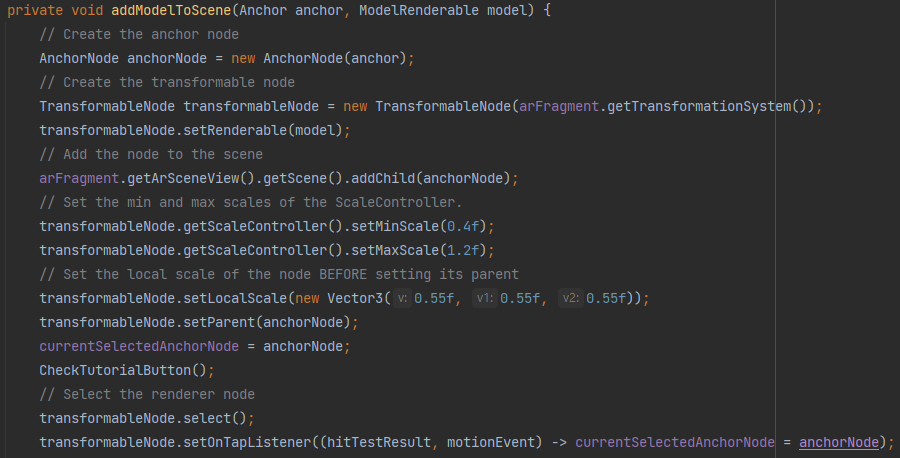
\includegraphics[width=0.8\textwidth]{img/code/addModelToScene.png}
    \caption{addModelToScene method}
    \label{fig:addModeltoScene}
\end{figure}

If a model is selected and the user wants to remove that model from the scene, he can do that by pressing the remove button. This will call the removeAnchorNode method, as seen in Figure \ref{fig:removeAnchorNode}. It will remove the model from the scene, and it will set the \textit{selectedModel} variable to null.

\begin{figure}[H]
    \centering
    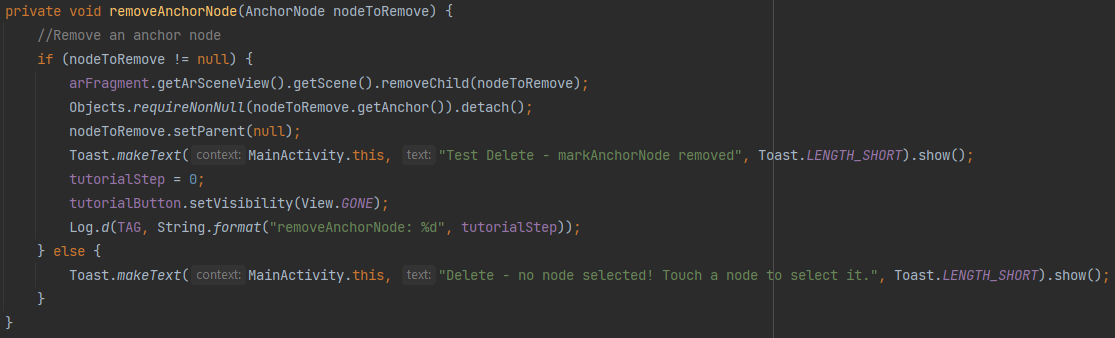
\includegraphics[width=1\textwidth]{img/code/removeAnchorNode.png}
    \caption{removeAnchorNode method}
    \label{fig:removeAnchorNode}
\end{figure}

%%%%%%%%%%%%%%%%%%%%%%%%%%%%%%%%%%%%%%%%%%%%%%%%%
%%%%%%%%%%%% cap: intro %%%%%%%%%%%%%%%%%
%%%%%%%%%%%%%%%%%%%%%%%%%%%%%%%%%%%%%%%%%%%%%%%%%

\chapter{Conclusion}\label{cap:conclusion}
In the concluding chapter, we will summarize the main results of the thesis and we will present future work.
\section{Summary}
\section{Future work}
\cite[Testing]{CormenIA}


\chapter{Conclusion}\label{cap:conclusion}
In the concluding chapter, we will summarize the main results of the thesis and we will present future work.
\section{Summary}
\section{Future work}
In this section we will present the future work that will be done to improve the application.



\bibliographystyle{alpha}
\bibliography{mybib}

\addcontentsline{toc}{chapter}{Bibliography}

\end{document}